\documentclass[12pt]{article}

% Packages
\usepackage[margin=0.6in]{geometry}
\usepackage{graphicx}
\usepackage{amsmath}
\usepackage{float}
\usepackage[dvipsnames]{xcolor}
\usepackage{etoolbox}
\usepackage{soul}
\usepackage{multirow}
\usepackage[font=small,skip=0pt]{caption}
%\usepackage{tcolorbox}
%\definecolor{block-gray}{gray}{0.85}

\pagestyle{plain}


\begin{document}

\title{Solution ark \#2.\\ Stratified sampling}
\author{O\u{g}uz--Alper, Melike \& Pekarskaya, Tatsiana, Statistics Norway}
\maketitle

\section*{Exercise 0}

\begin{enumerate}
\item Explain in your own words what is stratified sample?\\
\fcolorbox{black}{ForestGreen!20}{
\begin{minipage}[t]{0.97\linewidth} 
\textbf{Solution:}
``Probability sampling method in which population units are partitioned into strata, and then a SRS is taken from each stratum" \hfill (Lohr, 2019, p.100)
\begin{figure}[H]
\begin{center}
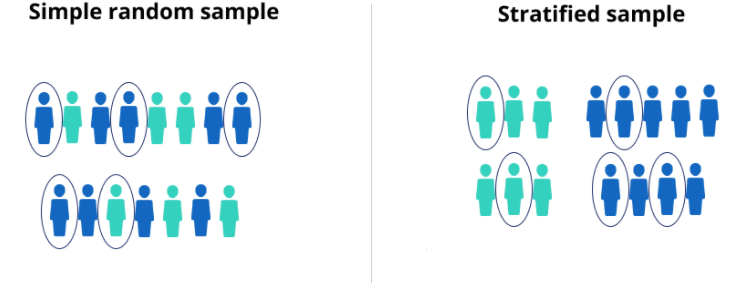
\includegraphics[scale=0.6]{SSRSvsSRS.png}
\end{center}
\caption{Source of the figure: https://www.scribbr.com/methodology/sampling-methods/}
\end{figure}
\end{minipage}}
\item What can be reasons to use a stratified sample rather than SRS?\\
\fcolorbox{black}{ForestGreen!20}{
\begin{minipage}[t]{0.97\linewidth} 
\textbf{Solution:}
`` We use stratified sampling for one or more of the following reasons:
\begin{enumerate}
\item We want to be protected from the possibility of obtaining a really bad sample. When taking an SRS of size 100 from a population of 1000 male and 1000 female students, obtaining a sample with no or very few males is theoretically possible, although such a sample in not likely to occur. Most people would not consider such a sample to be representative of the population and would worry that men and women might respond differently on the item of interest... 
\item We may want data of known precision from subgroups of the population. These subgroups should be strata. Mcllwee and Robinson (1992) sampled graduates from electrical and mechanical engineering programs at public university in southern California. They were interested in comparing the educational and workforce experience of male and female graduates, so they stratified their sampling frame by gender and took separate random samples of male and females graduates. Because there were many more male than female graduates, they sampled a higher fraction of female graduates than male graduates in order to obtain comparable precisions for the two groups.
\end{enumerate}
\end{minipage}}\\
\fcolorbox{black}{ForestGreen!20}{
\begin{minipage}[t]{0.97\linewidth} 
\begin{enumerate}
\setcounter{enumii}{2}
\item A stratified sample may be more convenient to administer and may result in a lower cost for the survey. For example, sampling frame may be constructed differently in different strata, or different sampling designs or field procedures may be used...
\item Stratified sampling often gives more precise (having lower variance) estimates for population means and totals. Persons of different ages tend to have different blood pressures, so in a blood pressure study it would be helpful to stratify by age groups..."
\end{enumerate}
 \hfill (Lohr, 2019, p.74)
\end{minipage}}

\end{enumerate}

\section*{Exercise 1}

Consider a population of 6 students. Suppose we know the test scores of the students to be
\begin{center}
\begin{tabular}{lrrrrrrr}
Student & \vline & 1& 2& 3& 4& 5& 6\\
\hline
Score & \vline &  66& 59& 70& 83& 82& 71\\
\end{tabular}
\end{center}
\begin{enumerate}
\item Find the mean $\bar{y}_U$ and variance $S^2$ of the population.\\
\fcolorbox{black}{ForestGreen!20}{
\begin{minipage}[t]{0.97\linewidth} 
\textbf{Solution:}
$\bar{y}_U = \frac{1}{N}\sum_{U}y_i = 71.83333$ and $S^2 = \frac{1}{N - 1}\sum_{U}(y_i - \bar{y}_U)^2 = 86.16667$
\end{minipage}}
\item How many SRS’s of size $4$ are possible?\\
\fcolorbox{black}{ForestGreen!20}{
\begin{minipage}[t]{0.97\linewidth} 
\textbf{Solution:}
$\binom{6}{4}= C_6^4 =6!/(4!2!)=15$ possible samples of size $n=4$ 
\end{minipage}}
\item List the possible SRS’s. For each, find the sample mean. Find sampling variance $V(\bar{y})$, using $$V(\bar{y})=(1-n/N)n^{-1}S^2\cdot$$\\
\fcolorbox{black}{ForestGreen!20}{
\begin{minipage}[t]{0.97\linewidth} 
\textbf{Solution:}
$15$ possible samples and $\bar{y}_S$ are given below. Sample mean we find by formula $\bar{y}_S = \frac{1}{n_S}\sum_{S}y_i$
\begin{center}
\renewcommand{\tabcolsep}{0.1cm}
\begin{tabular}{cccccccc}
$S$ & $\bar{y}_S$ &\vline & $S$ & $\bar{y}_S$ & \vline & $S$ & $\bar{y}_S$ \\
\hline
$S_1$=\{1,2,3,4\} &69.50 &\vline &$S_6$=\{1,2,5,6\} &69.50 &\vline &$S_{11}$=\{2,3,4,5\}&73.50 \\
$S_2$=\{1,2,3,5\} & 69.25&\vline &$S_7$=\{1,3,4,5\} & 75.25&\vline &$S_{12}$=\{2,3,4,6\}&70.75 \\
$S_3$=\{1,2,3,6\} & 66.50&\vline &$S_8$=\{1,3,4,6\} & 72.50&\vline &$S_{13}$=\{2,3,5,6\}& 70.50\\
$S_4$=\{1,2,4,5\} & 72.50&\vline &$S_9$=\{1,3,5,6\} &72.25 &\vline &$S_{14}$=\{2,4,5,6\}&73.75 \\
$S_5$=\{1,2,4,6\} & 69.75&\vline &$S_{10}$=\{1,4,5,6\} &75.50 &\vline &$S_{15}$=\{3,4,5,6\}&76.50 \\
\end{tabular}
\end{center}
$$V(\bar{y})=\Big(1-\frac{4}{6}\Big)\frac{86.17}{4}=7.18$$
\end{minipage}}
\item Now let stratum one consist of students 1–3, and stratum two consist of students 4–6. How many stratified random samples of size $4$ are possible in which $2$ students are selected from each stratum?\\
\fcolorbox{black}{ForestGreen!20}{
\begin{minipage}[t]{0.97\linewidth} 
\textbf{Solution:}
There are $\binom{3}{2}\binom{3}{2}=9$ possible  
\end{minipage}}
\item List the possible stratified random samples. Which of the samples from (3) cannot occur with the stratified design defined in (4)?\\
\fcolorbox{black}{ForestGreen!20}{
\begin{minipage}[t]{0.97\linewidth} 
\textbf{Solution:}
$9$ possible stratified samples of size $n_h=2$ from each stratum:
\begin{center}
\begin{tabular}{cccccccc}
$S$ & $\bar{y}_{str}$ &\vline & $S$ &$\bar{y}_{str}$& \vline & $S$&$\bar{y}_{str}$  \\
\hline
\{1,2,4,5\} &72.50 & \vline &\{1,3,4,5\} &75.25&\vline &\{2,3,4,5\} &73.50 \\
\{1,2,4,6\} &69.75&\vline &\{1,3,4,6\} &72.50&\vline &\{2,3,4,6\} &70.75\\
\{1,2,5,6\} &69.50& \vline &\{1,3,5,6\} &72.25&\vline &\{2,3,5,6\} &70.50 \\
\end{tabular}
\end{center}
Samples $S_1,S_2,S_3,S_{10},S_{14},S_{15}$ cannot occur with the stratified sampling given as they include three units from one of the strata: \{1,2,3\} or \{4,5,6\}. 
\end{minipage}}
\item Find $\bar{y}_{str}$ for each possible stratified random sample. Find $V(\bar{y}_{str})$, and compare it to $V(\bar{y})$.\\
\fcolorbox{black}{ForestGreen!20}{
\begin{minipage}[t]{0.97\linewidth} 
\textbf{Solution:}
Use  $$\bar{y}_{str}=\frac{1}{N}\sum_{H}N_h\bar{y}_h,$$ where $N=6$, $N_h=3$ and $n_h=2$, for all $h$ in $H$. Results of calculations of $\bar{y}_{str}$, one can find in (5).\\
Further we calculate $$V(\bar{y}_{str})=\sum_{H}(1-f_h)(\frac{N_h}{N})^2 \frac{1}{n_h}S_h^2,$$
where $f_h=n_h/N_h$ and  $S_h^2 = \sum_{j=1}^{N_h}\frac{(y_{hj} - \bar{y}_{hU})}{N_h - 1}.$ 
We have $S_1^2 = 31$ and $S_2^2 = 44.3333$, with $h \in \{1,2\}$.
$$V(\bar{y}_{str})=\Big(1-\frac{2}{3}\Big)\,\Big(\frac{3}{6}\Big)^2\,\frac{1}{2}\, 31 + \Big(1-\frac{2}{3}\Big)\,\Big(\frac{3}{6}\Big)^2\,\frac{1}{2}\, 44.3333=3.14	$$ 
$V(\bar{y}_{str})$ is much smaller than $V(\bar{y})$ as units within strata are more alike than units without stratification, so that we have $S_1^2< S^2$ and $S_2^2<S^2$.
\end{minipage}} 
\end{enumerate}

\section*{Exercise 2}
A stratified sample is being designed to estimate the prevalence p of a rare characteristic,
say the proportion of residents in Milwaukee, Wisconsin, who have Lyme
disease. Stratum one, with $N_1$ units, has a high prevalence of the characteristic; stratum
two, with $N_2$ units, has low prevalence. Assume that the cost to sample a unit (for
example, the cost to select a person for the sample and determine whether he or she
has Lyme disease) is the same for each stratum, and that at most $2\,000$ units are to be
sampled.
\begin{enumerate}
\item  Let $p_1$ and $p_2$ be the proportions in stratum one and stratum two with the rare characteristic.
If $p_1=0.10$, $p_2=0.03$, and $N_1/N = 0.4$, what are $n_1$ and $n_2$ under optimal allocation?\\
\fcolorbox{black}{ForestGreen!20}{
\begin{minipage}[t]{0.97\linewidth} 
\textbf{Solution:}
Let $p_1=0.1$, $p_2=0.03$, and $N_1/N=0.4$. Find $n_h$ under optimal allocation. We use $n_h=nN_hS_h/\sum_{h}N_hS_h$.
$$S_1=\sqrt{p_1(1-p_1)}=\sqrt{0.1*0.9} = 0.3, S_2=\sqrt{0.03*0.97} = 0.1706\cdot$$
$$\sum_{h}N_hS_h=0.3*0.4N + 0.1706 *0.6N= 0.12N+0.1024N=0.2224N$$
$$n_1=2\,000\frac{0.12}{0.2224}=1\,079 \quad n_2=2\,000\frac{0.1024}{0.2224}=921$$
\end{minipage}}
\item If $p_1=0.10$, $p_2=0.03$, and $N_1/N = 0.4$, what is $V(\hat{p}_{str})$ under proportional allocation? Under optimal allocation? What is the variance if you take an SRS of $2\,000$ units from the population? \\
\fcolorbox{black}{ForestGreen!20}{
\begin{minipage}[t]{0.97\linewidth} 
\textbf{Solution:}
Let $p_1=0.1$, $p_2=0.03$, and $N_1/N=0.4$. Find $V_{opt}(\hat{p}_{str})$ and $V_{prop}(\hat{p}_{str})$ under optimal and proportional allocations, respectively. Find also $V_{srs}(\hat{p}_{str})$. Suppose $f_h\approx 0$. \\
With optimal allocation:
$$V_{opt}(\hat{p}_{str})=0.4^2\frac{0.1*0.9}{1\,079}+0.6^2\frac{0.03*0.97}{921}=2.47\times 10^{-5}$$
With proportional allocation: 
$$n_1=2\,000*0.4=800 \quad n_2=2\,000*0.6=1\,200$$
$$V_{prop}(\hat{p}_{str})=0.4^2\frac{0.1*0.9}{800}+0.6^2\frac{0.03*0.97}{1\,200}=2.67\times 10^{-5}$$
Under SRS, we have $p=0.4*0.1+0.6*0.03=0.058$.
$$V_{srs}(\hat{p}_{str})=\frac{0.058*(1-0.058)}{2\,000}=2.73\times 10^{-5}$$
$V_{opt}(\hat{p}_{str})<V_{prop}(\hat{p}_{str})<V_{srs}(\hat{p}_{str})$.

\end{minipage}}
\end{enumerate}

\section*{Exercise 3}
\textbf{\color{ForestGreen}(R code available)} Consider the same problem as in exercise 4 previous section. In the SRS of 50 faculty members not all the departments were represented. The SRS contained several faculty members from psychology and from chemistry but none from the foreign languages. It was therefore decided to take a stratified simple random sample, using the areas biological sciences, physical sciences, social sciences and humanities as the strata. Proportional allocation was used in this sample. The distribution of the strata for population and sample are given below
	
\begin{center}
\begin{tabular}{lcc}
Stratum & Number of faculty & Number of faculty members\\
& members in the stratum & in the samples\\
\hline
1 - Biological sciences & 102 & 7\\
2 - Physical sciences & 310 & 19\\
3 - Social sciences & 217 & 13\\
4 - Humanities & 178 & 11\\
\hline
Total & 807 & 50\\
\end{tabular}
\end{center}

The data from the stratified sample turned out to be
\begin{center}
\begin{tabular}{c|cccc}
Number of & Number of refereed publications \\
faculty members & Biological & Physical & Social & Humanities\\
\hline
0&	1	&10	&9	&8\\
1&	2	&2	&0	&2\\
2&	0	&0	&1	&0\\
3&	1	&1	&0	&1\\
4&	0	&2	&2	&0\\
5&	2	&1	&0	&0\\
6&	0	&1	&1	&0\\
7&	1	&0	&0	&0\\
8&	0	&2	&0	&0\\

\end{tabular}
\end{center}

\begin{enumerate}
\item Estimate the total number of refereed publications by faculty members in the college and compute the standard error.\\
\fcolorbox{black}{ForestGreen!20}{
\begin{minipage}[t]{0.97\linewidth} 
%%%Ex 3 a
\textbf{Solution:}

The total number of publications by department in the sample:
%\small
\begin{center}
\begin{tabular}{cccccc}
 &\vline & Biological & Physical & Social & Humanities\\
 \hline
Total number of  &\vline & \multirow{2}{*}{22} & \multirow{2}{*}{40} & \multirow{2}{*}{16} & \multirow{2}{*}{5} \\
refereed publications & \vline &  &  &  & \\
\hline
\end{tabular}
\end{center}

The total number of publications is estimated by
$$\hat{t}_{str}=\sum_{h}N_h\bar{y}_h$$ and its standard error is estimated by 
$$\widehat{SE}(\hat{t}_{str})=\sqrt{\sum_{h}N_h^2\,(1-f_h)\,\frac{s_h^2} {n_h}}\cdot$$
$$\hat{t}_{str}=102\frac{22}{7}+310\frac{40}{19}+217\frac{16}{13}+178\frac{5}{11}=1\,312.189$$
We have\\
$s_1^2=6.809524$, $s_2^2=8.210526$, $s_3^2=4.358974$, and $s_4^2=0.872727$.

\begin{eqnarray*}
\hat{V}_{str}(\hat{t}_{str})&=&102^2\Big(1-\frac{7}{102}\Big)\frac{6.8095}{7}+310^2\Big(1-\frac{19}{310}\Big)\frac{8.2105}{19} + 217^2\Big(1-\frac{13}{217}\Big)\frac{4.3590}{13} + \\
&&\\
&&+178^2\Big(1-\frac{11}{178}\Big)\frac{0.8727}{11} = 65\,610.78\\
\end{eqnarray*}
$$\widehat{SE}(\hat{t}_{str})=\sqrt{\hat{V}_{str}(\hat{t}_{str})}=\sqrt{65\,610.78}=256.15.$$
\end{minipage}}
\item How does the result from part (1) compare with the result from the SRS in Exercise 4 previous session?\\
\fcolorbox{black}{ForestGreen!20}{
\begin{minipage}[t]{0.97\linewidth} 
\textbf{Solution:}
%%%Ex3 3
In Exercise 4 of Session 1, we had an SRS of faculty members, and $\bar{y}=1.78$ and $\widehat{SE}(\bar{y})=0.367$. Thus, we find
$$\hat{t}_{srs}=N\bar{y}=807*1.78=1\,436.46,\quad \widehat{SE}(\hat{t}_{srs}) = 807*0.367=296.12.$$
\begin{itemize}
\item Stratified sampling ensures that each department is represented in the sample
\item Smaller standard error with stratified sampling as units within stratum tend to be more homogeneous than the units in the population as a whole. We had $s^2=7.1955$ under SRS. Note that $s_1^2,s_3^2,s_4^2<s^2$ and $s_2^2>s^2$.
\end{itemize}

\end{minipage}}
\item Estimate the proportion of faculty with no refereed publications and compute the standard error and 95\% confidence interval.\\
\fcolorbox{black}{ForestGreen!20}{
\begin{minipage}[t]{0.97\linewidth} 
\textbf{Solution:}
%%%Ex3 4
\begin{center}
\begin{tabular}{ccrrrr}
 &\vline & Biological & Physical & Social & Humanities\\
 \hline
 $N_h$  &\vline & 102 & 310 & 217 & 178\\
$n_h$  &\vline & 7 & 19 & 13 & 11\\
$\#$ of publications  & \vline & \multirow{2}{*}{1} & \multirow{2}{*}{10} & \multirow{2}{*}{9} & \multirow{2}{*}{8} \\
 with no references & \vline &  & &  &  \\
\hline
\end{tabular}
\end{center}
The proportion of faculty with no publications is estimated by\\
$$\hat{p}_{str}=\sum_{h}N_h\hat{p}_h/N =\frac{1}{807}(102\,\frac{1}{7}+310\,\frac{10}{19}+217\,\frac{9}{13}+178\,\frac{8}{11}\Big) = 0.5668$$

$$\hat{V}_{str}(\hat{p}_{str})=N^{-2}\sum_{h}N_h^2\,(1-f_h)\,\hat{p}_h\,(1-\hat{p}_h)(n_h-1)^{-1},$$
where \\
$\hat{p}_1=1/7=0.1429, \hat{p}_2=10/19 = 0.5263,$ \\
$\hat{p}_3=9/13=0.6923, \hat{p}_4=8/11=0.7273,$

with $h \in \{1,2,3,4\}$.
$$\hat{V}_{str}(\hat{p}_{str})=0.0003+0.0019+0.0012+0.0009=0.0043,$$
$$\widehat{SE}(\hat{p}_{str})=\sqrt{0.0043}=0.066\cdot$$

\end{minipage}}
\item Compare the result in part (3) with the result from the SRS in Exercise 4 previous session.\\
\fcolorbox{black}{ForestGreen!20}{
\begin{minipage}[t]{0.97\linewidth} 
\textbf{Solution:}
Under SRS (see Exercise 4 of Session 1), we had $\hat{p}_{srs}=0.56$ and $SE(\hat{p}_{srs})=0.069$. Not so much gain in precision from stratified sampling design in comparison to SRS design. 
\end{minipage}}
\item Did the stratification increase precision for the two estimation problems considered in parts (1) and (3) ? Explain why you think it did or did not.\\
\fcolorbox{black}{ForestGreen!20}{
\begin{minipage}[t]{0.97\linewidth} 
\textbf{Solution:}
Yes, precision was increased, since SE is smaller and CI is shorter.
\end{minipage}}
\end{enumerate}

\section*{Exercise 4}
A public opinion researcher has a budget of \$20 000 for taking a survey. She knows that 90\% of all households have known telephone numbers. Telephone interviews cost \$10 per household; in-person interviews cost \$30 each if all interviews are conducted in person and \$40 each if only households with unknown telephone numbers are interviewed in person (because there will be extra travel costs). Assume that the variances in phone and nonphone strata are similar and that the fixed costs are $c_0 = \$5\,000$.  
\begin{enumerate}
\item How many households should be interviewed in each group if all households are interviewed in person?\\
\fcolorbox{black}{ForestGreen!20}{
\begin{minipage}[t]{0.97\linewidth} 
\textbf{Solution:}
Find $n$ if all households interviewed in person. \\
$C=c_0+\sum_{h}c_h n_h$, with $C=20\,000$ and $c_0=5\,000$, thus $\sum_{h}c_h n_h=15\,000$. Since costs are the same, we have\\
$30n=15\,000 \implies n=500$, with $n=\sum_{h}n_h$.
Formula for $n_h$ by using optimal allocation:
$$n_h=n\frac{N_hS_h/\sqrt{c_h}}{\sum_{h}N_hS_h/\sqrt{c_h}}$$
\end{minipage}}\\
\fcolorbox{black}{ForestGreen!20}{
\begin{minipage}[t]{0.97\linewidth} 
Since variances are similar in strata and costs are the same, optimal allocation results in proportional allocation. \\
Using $n_h=n N_h/N$, $N_1/N=0.9$ and $N_2/N=0.1$, we obtain\\ $n_1=0.9*500=450$ and $n_2=0.1*500=50$,\\
where $n_1$ and $n_2$ are sample sizes for phone and nonphone households, respectively.
\end{minipage}}
\item How many households should be interviewed in each stratum if households with a known telephone number are contacted by telephone and the other households are contacted in person?\\
\fcolorbox{black}{ForestGreen!20}{
\begin{minipage}[t]{0.97\linewidth} 
\textbf{Solution:}
The sample size per stratum with optimal allocation given similar $S_h$ is given by
$$n_h=n\frac{N_h/\sqrt{c_h}}{\sum_{h}N_h/\sqrt{c_h}}$$
$$\sum_{h}N_h/\sqrt{c_h}=0.9N/\sqrt{10}+0.1N/\sqrt{40}=0.300416N.$$
Using $\sum_{h}c_h n_h=15\,000$, we obtain
$$\frac{1}{0.300416}(10n\,0.9/\sqrt{10}+40n\,0.1/\sqrt{40})=15\,000\cdot$$
\begin{itemize}
\item $n=1\,295,$
\item $n_1=1\,295*0.9/\sqrt{10}/0.300416=1\,227,$
\item $n_2=1\,295*0.1/\sqrt{40}/0.300416=68.$
\end{itemize}
Thanks to the reduced costs of telephone interviewing, the sample size becomes larger.
\end{minipage}}
\item Which of the two data collection methods would you choose? Give a justification for your answer.\\
\fcolorbox{black}{ForestGreen!20}{
\begin{minipage}[t]{0.97\linewidth} 
\textbf{Solution:}
Collection method described in 2 is better, since provides possibility to survey more households. 
\end{minipage}}\\
\end{enumerate}

\section*{Exercise 5}
Burnard (1992) sent a questionnaire to a stratified sample of nursing tutors and students in Wales, to study what the tutors and students understood by the term \emph{experiential learning}. The population size and sample size obtained for each of the four strata are
given below:
\begin{center}
\begin{tabular}{lrr}
Stratum & Population size & Sample size \\
\hline
General nursing tutors (GT) &150 &109\\
Psychiatric nursing tutors (PT)&34 &26\\
General nursing students (GS) &2 680& 222\\
Psychiatric nursing students (PS)&570& 40\\
\hline
Total & 3\,434 &397 \\
\end{tabular}
\end{center}
Respondents were asked which of the following techniques could be identified as experiential learning methods; the number of students in each group who identified
the method as an experiential learning method are given below:
\begin{center}
\begin{tabular}{lrrrrr}
Method & \vline & GS & PS & PT & GT \\
\hline
Role play &\vline & 213 &38& 26 &104\\
Problem solving activities&\vline & 182& 33& 22& 95\\
Simulations &\vline &95 &20 &22 &64\\
Empathy-building exercises &\vline &89 &25& 20& 54\\
Gestalt exercises &\vline &24& 4& 5& 12\\ 
\end{tabular}
\end{center}
Estimate the overall percentage of nursing students and tutors who identify ``Role play" techniques as “experiential learning”. Be sure to give standard errors for your estimate.
\\
\fcolorbox{black}{ForestGreen!20}{
\begin{minipage}[t]{0.97\linewidth} 
\textbf{Solution:}
Using $$\hat{p}_{str}=\sum_{h}N_h\hat{p}_h/N$$ and $$\widehat{SE}(\hat{p}_{str})=\sqrt{\sum_{h}\frac{1}{N^2} N_h^2(1-f_h)\hat{p}_h(1-\hat{p}_h)\frac{1}{n_h-1}},$$ \\
we obtain for ``Role play":
$\hat{p}_{str}=\frac{1}{3\,434}\Big(2\,680\frac{213}{222}+570\frac{38}{40}+34\frac{26}{26}+150\frac{104}{109}\Big)=0.96$\\
$\widehat{SE}(\hat{p}_{str})=\sqrt{\frac{1}{3\,434^2}\Big[2\,680^2(1-0.083)\frac{213}{222}\Big(1-\frac{213}{222}\Big)\frac{1}{221}+\cdots\Big]}=0.011$

\end{minipage}}
\end{document}